\documentclass[11pt]{article}

% "final" = camera-ready look with author names (no line numbers)
\usepackage[final]{acl}

\usepackage{times}
\usepackage{latexsym}
\usepackage[T1]{fontenc}
\usepackage[utf8]{inputenc}
\usepackage{microtype}
\usepackage{inconsolata}
\usepackage{graphicx}
\usepackage{booktabs}
\usepackage{amsmath}
\usepackage{amssymb}

\title{Parameter-Efficient Fine-Tuning Showdown:\\Full Fine-Tuning vs LoRA vs Adapters vs Prompt Tuning\\[4pt]\large Team 18 (P18), Deep Learning Project Report}

\author{Deepak Mandal \\ su-24039@sitare.org \And
  Anoop Kumar \\ su-24017@sitare.org \AND
  Chiranjeet Biswas \\ su-24037@sitare.org \And
  Byagari Praveen Kumar \\ su-24034@sitare.org}

\begin{document}
\maketitle

\begin{abstract}
We compare four ways of adapting \texttt{roberta-base} to a classification task: full fine-tuning (Full FT), LoRA, bottleneck adapters and prompt tuning. Every method uses the same data splits, seeds, sequence length, batch size, epochs and GPU type. We report accuracy (and F1 on MRPC), trainable parameters, peak GPU memory, training time and checkpoint size on GLUE SST-2, MRPC and RTE, with the full training set and with only 1,000 training examples. The study has 122 training runs: 64 for the main grid, 16 for a learning-rate search and 42 for ablations. Adapters are tied with Full FT on accuracy while training 1.9\% of the parameters and using 42\% less peak GPU memory. LoRA is 0.3--2.1 points behind Full FT with 0.71\% of the parameters and a 3.4\,MB checkpoint. With 1,000 examples, Full FT and adapters lose the least accuracy. Prompt tuning stays close to the majority-class baseline on MRPC and RTE at this model size, as predicted by \citet{lester2021}. Code and all result files: \url{https://github.com/Anoop1230-tech/peft-showdown}.
\end{abstract}

\section{Introduction}

Full fine-tuning updates every weight of a pretrained model. For each new task this means storing another full copy of the model (about 500\,MB for \texttt{roberta-base}) and keeping optimizer state for all 125M parameters in GPU memory. Parameter-efficient fine-tuning (PEFT) methods freeze the pretrained weights and train only a small number of new or selected parameters.

Published comparisons often differ in base model, training budget, or how trainable parameters are counted (for example, whether the classification head is included). We compare full fine-tuning, LoRA \citep{hu2022}, adapters \citep{houlsby2019} and prompt tuning \citep{lester2021} under one fixed setup on three GLUE tasks \citep{wang2019}. We answer four questions: how close each PEFT method gets to Full FT and at what parameter cost; which method loses the least accuracy with only 1,000 training examples; why prompt tuning is weak at this model size; and which method to use under a memory limit, a time limit or very little data.

\section{Background}

\paragraph{Adapters.} \citet{houlsby2019} insert small bottleneck MLPs into every transformer layer: a down-projection to dimension $m$, a nonlinearity, an up-projection back to the hidden size $d$, and a residual connection. The Houlsby variant places one adapter after the attention block and one after the feed-forward block. \citet{pfeiffer2021} use a single adapter after the feed-forward block. Houlsby et al.\ reach within 0.4\% of full fine-tuning on GLUE while training about 3.6\% of the parameters per task.

\paragraph{LoRA.} For a frozen weight matrix $W_0 \in \mathbb{R}^{d\times k}$, LoRA \citep{hu2022} learns a low-rank update, so the layer computes $W_0x + \frac{\alpha}{r}BAx$ with $B \in \mathbb{R}^{d\times r}$, $A \in \mathbb{R}^{r\times k}$ and a small rank $r$. $B$ starts at zero, so training starts from the pretrained model, and after training $BA$ can be merged into $W_0$, so inference costs nothing extra.

\paragraph{Prompt tuning.} \citet{lester2021} freeze the model and prepend $p$ learnable ``virtual token'' embeddings to the input. Only these embeddings are trained. With T5 they show that the gap to full fine-tuning is large for small models and closes only at around 10B parameters.

\section{Methods}

All methods use \texttt{roberta-base} \citep{liu2019} (12 layers, hidden size 768) with RoBERTa's classification head (a $768{\times}768$ dense layer with tanh and a $768{\times}2$ projection, 592,130 parameters). The head is trained in every method and counted in every trainable-parameter number. Table~\ref{tab:methods} lists the method settings. LoRA and prompt tuning use Hugging Face \texttt{peft} 0.21.2. \texttt{peft} has no Houlsby adapters, so adapters use AdapterHub \texttt{adapters} 1.3.0, built on the same \texttt{transformers} models.

\begin{table}[t]
\centering
\small
\begin{tabular}{@{}lrrl@{}}
\toprule
Method & Trainable & \% & LR \\
\midrule
Full FT & 124,647,170 & 100.00 & 2e-5 \\
LoRA ($r{=}8$, $\alpha{=}16$, q/v) & 887,042 & 0.71 & 5e-4 \\
Adapters (Houlsby, $m{=}48$) & 2,381,186 & 1.87 & 3e-4 \\
Prompt tuning (20 tokens) & 607,490 & 0.48 & 1e-2 \\
\bottomrule
\end{tabular}
\caption{Methods, trainable parameters (head included) and learning rates. LoRA uses dropout 0.1 on the query and value projections of all 12 layers. Adapters use reduction factor 16 (24 adapters). Prompt tuning uses random initialisation.}
\label{tab:methods}
\end{table}

\section{Experimental Setup}

\paragraph{Same budget.} AdamW, weight decay 0.01, linear warmup over 6\% of the steps, batch size 32, maximum sequence length 128, fp16. Epochs: 3 for SST-2 full data, 10 for MRPC and RTE full data, 20 for every 1k run. Only the method-specific settings and the learning rate differ.

\paragraph{Splits.} GLUE test labels are hidden, so we report on the official validation split. We hold out 10\% of the training set as our dev split. The checkpoint with the best dev accuracy (evaluated every epoch) is kept, and the LR search also uses the dev split. The validation split is never used for any choice.

\paragraph{Low-data regime.} 1,000 examples are drawn from the training part with the run's seed, so every method sees the same examples for a given seed.

\paragraph{Seeds and measurements.} Seeds 1, 2 and 3 for every configuration, except SST-2 full data (seed 1 only, about one hour per Full FT run). We record trainable parameters (\texttt{requires\_grad}, head included), peak GPU memory (\texttt{torch.cuda.max\_memory\_allocated} after resetting the peak counter), wall-clock training time and the size of the saved trainable weights. Each run is a separate process on one Tesla T4 (16\,GB) on Kaggle.

\paragraph{Learning-rate search.} Following our plan, we tried three learning rates per method with seed 1 on RTE and MRPC full data. For every method, the learning rate used in the final runs had the best mean dev accuracy (Table~\ref{tab:lr}), so the final runs did not need to be repeated.

\begin{table}[t]
\centering
\small
\begin{tabular}{@{}llrrr@{}}
\toprule
Method & LR & RTE & MRPC & Mean \\
\midrule
Full FT & 1e-5 & 76.7 & \textbf{88.3} & 82.5 \\
 & 2e-5* & \textbf{78.3} & 87.2 & \textbf{82.8} \\
 & 3e-5 & \textbf{78.3} & 86.9 & 82.6 \\
\midrule
LoRA & 1e-4 & 70.7 & 86.9 & 78.8 \\
 & 3e-4 & 74.7 & \textbf{88.6} & 81.7 \\
 & 5e-4* & \textbf{75.9} & 88.3 & \textbf{82.1} \\
\midrule
Adapters & 1e-4 & 71.1 & 86.9 & 79.0 \\
 & 3e-4* & \textbf{77.9} & 87.5 & \textbf{82.7} \\
 & 1e-3 & 75.9 & \textbf{88.0} & 82.0 \\
\midrule
Prompt & 1e-3 & 52.2 & 69.2 & 60.7 \\
tuning & 1e-2* & \textbf{55.8} & 72.8 & \textbf{64.3} \\
 & 3e-2 & 52.2 & \textbf{73.8} & 63.0 \\
\bottomrule
\end{tabular}
\caption{LR search: dev accuracy ($\times$100), seed 1, full data. * = LR used in all final runs.}
\label{tab:lr}
\end{table}

\section{Results}

\begin{table*}[t]
\centering
\resizebox{\textwidth}{!}{%
\begin{tabular}{@{}lcccccccc@{}}
\toprule
Method & SST-2 full & SST-2 1k & MRPC full & MRPC full F1 & MRPC 1k & MRPC 1k F1 & RTE full & RTE 1k \\
\midrule
Full FT & 94.0 & 90.4 $\pm$ 0.5 & 87.7 $\pm$ 1.4 & 91.2 $\pm$ 1.2 & 85.8 $\pm$ 2.2 & 89.9 $\pm$ 1.4 & 76.1 $\pm$ 2.2 & 69.9 $\pm$ 2.1 \\
LoRA & 93.7 & 90.1 $\pm$ 0.5 & 87.1 $\pm$ 1.0 & 90.9 $\pm$ 0.6 & 84.3 $\pm$ 1.3 & 88.8 $\pm$ 0.9 & 74.0 $\pm$ 2.0 & 66.9 $\pm$ 3.2 \\
Adapters & 94.2 & 90.4 $\pm$ 0.8 & 87.3 $\pm$ 0.6 & 91.0 $\pm$ 0.4 & 84.4 $\pm$ 1.0 & 89.1 $\pm$ 0.8 & 76.3 $\pm$ 1.8 & 71.2 $\pm$ 2.0 \\
Prompt tuning & 91.2 & 73.7 $\pm$ 15.4 & 70.7 $\pm$ 1.9 & 81.5 $\pm$ 0.7 & 71.1 $\pm$ 2.5 & 81.9 $\pm$ 1.0 & 56.1 $\pm$ 2.6 & 52.8 $\pm$ 2.7 \\
\textit{Majority class} & \textit{50.9} & \textit{50.9} & \textit{68.4} & \textit{81.2} & \textit{68.4} & \textit{81.2} & \textit{52.7} & \textit{52.7} \\
\midrule
 & Trainable & \% trainable & Peak mem (MiB) & Time RTE (s) & Time SST-2 (s) & Checkpoint (MB) & & \\
\midrule
Full FT & 124,647,170 & 100.00 & 3,264 & 158 & 492 & 475.5 & & \\
LoRA & 887,042 & 0.71 & 1,937 & 112 & 324 & 3.4 & & \\
Adapters & 2,381,186 & 1.87 & 1,884 & 106 & 378 & 9.1 & & \\
Prompt tuning & 607,490 & 0.48 & 1,923 & 117 & 385 & 2.3 & & \\
\bottomrule
\end{tabular}}
\caption{Unified comparison. Top: GLUE validation accuracy (and F1 on MRPC) $\times$100, mean $\pm$ std over seeds 1--3 (SST-2 full: seed 1 only). Bottom: efficiency; peak memory is the maximum over a method's runs, times on a Tesla T4 with full training data.}
\label{tab:main}
\end{table*}

\subsection{Unified comparison}

Table~\ref{tab:main} is the unified comparison and Figure~\ref{fig:params} plots accuracy against trainable parameters.

\paragraph{Adapters} are within $\pm$0.4 points of Full FT on every full-data score (94.2 vs 94.0 on SST-2, 87.3 vs 87.7 on MRPC, 76.3 vs 76.1 on RTE). All of these gaps are smaller than one standard deviation (1.4--2.2 points on MRPC and RTE), so the two methods are tied on accuracy. Adapters train 1.9\% of the parameters, use 42\% less peak memory (1,884 vs 3,264\,MiB) and train 33\% faster on RTE (106 vs 158\,s).

\paragraph{LoRA} is 0.3 points behind Full FT on SST-2, 0.6 on MRPC and 2.1 on RTE. It trains fewer parameters than adapters (0.89M vs 2.38M), has a smaller checkpoint (3.4 vs 9.1\,MB) and is the fastest method on SST-2 (324 vs 492\,s).

\paragraph{Prompt tuning} is far behind on the two small tasks. On MRPC, 70.7\% accuracy and 81.5 F1 are almost the same as always predicting ``paraphrase'' (68.4\% / 81.2). On RTE, 56.1\% is 3.4 points above the majority class. With the 67k SST-2 examples it reaches 91.2\%, so it does learn when it gets enough data.

\paragraph{Memory and time.} All PEFT methods use about 40\% less peak memory than Full FT because the optimizer only keeps state for the trainable parameters. They differ little from each other (1,884--1,937\,MiB), because the activations of the frozen backbone dominate. Prompt tuning makes every input 20 tokens longer, so it is not faster than LoRA or adapters despite training the fewest parameters.

\begin{figure}[t]
\centering
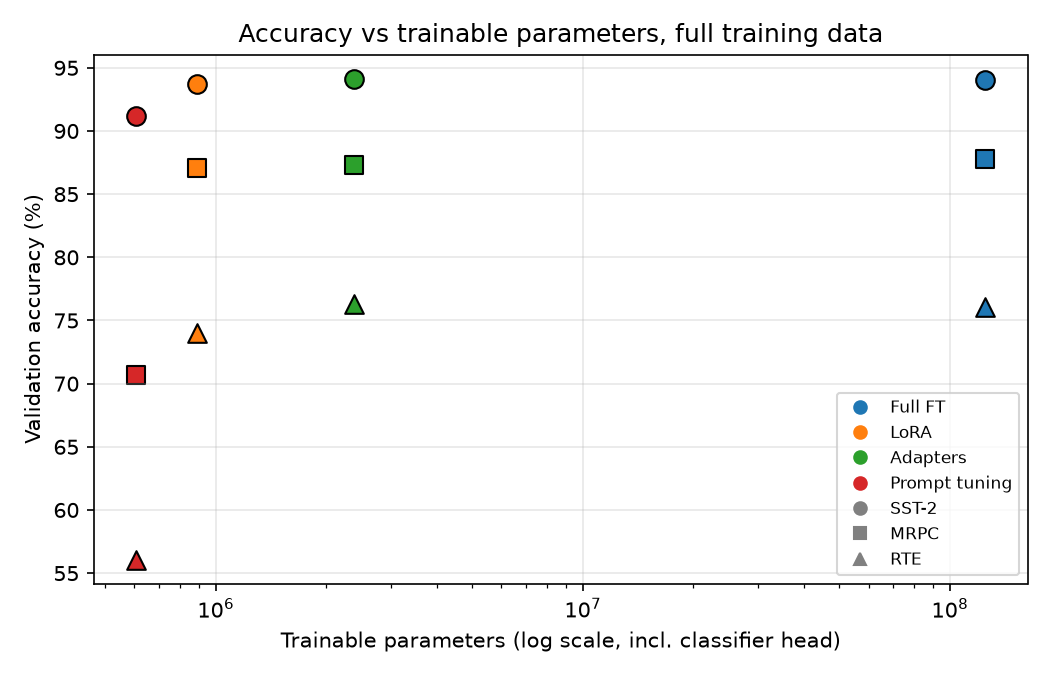
\includegraphics[width=\columnwidth]{figures/acc_vs_params.png}
\caption{Validation accuracy vs trainable parameters (log scale), one point per method and task, full training data.}
\label{fig:params}
\end{figure}

\subsection{Low-data regime}

\begin{table}[t]
\centering
\small
\begin{tabular}{@{}lrrrr@{}}
\toprule
Method & SST-2 & MRPC & RTE & Mean \\
\midrule
Full FT & $-$3.7 & $-$2.0 & $-$6.1 & 3.9 \\
LoRA & $-$3.6 & $-$2.8 & $-$7.1 & 4.5 \\
Adapters & $-$3.8 & $-$2.9 & $-$5.1 & 3.9 \\
Prompt tuning & $-$17.5 & +0.4 & $-$3.2 & 6.8 \\
\bottomrule
\end{tabular}
\caption{Accuracy change (points) from full data to 1,000 training examples, mean over seeds.}
\label{tab:lowdata}
\end{table}

Table~\ref{tab:lowdata} and Figure~\ref{fig:lowdata} show what happens with only 1,000 training examples. Full FT and adapters lose the least, 3.9 points on average. Adapters have the best RTE 1k score (71.2 vs 69.9 for Full FT), but their standard deviations (2.0 and 2.1) overlap, so we do not claim a clear winner. LoRA loses a bit more, mostly on RTE ($-$7.1, $\pm$3.2 across seeds).

Prompt tuning becomes unstable. On SST-2 1k, seeds 1 and 3 reach 83.7\% and 81.3\%, but seed 2 stays at 56.0\%, hence the $\pm$15.4 standard deviation. The best checkpoints of the working seeds were at epochs 17 and 20 of 20, so prompt tuning was still improving when training stopped. Its small drops on MRPC and RTE do not mean it holds up well: it was already near the majority-class baseline with full data.

\begin{figure}[t]
\centering
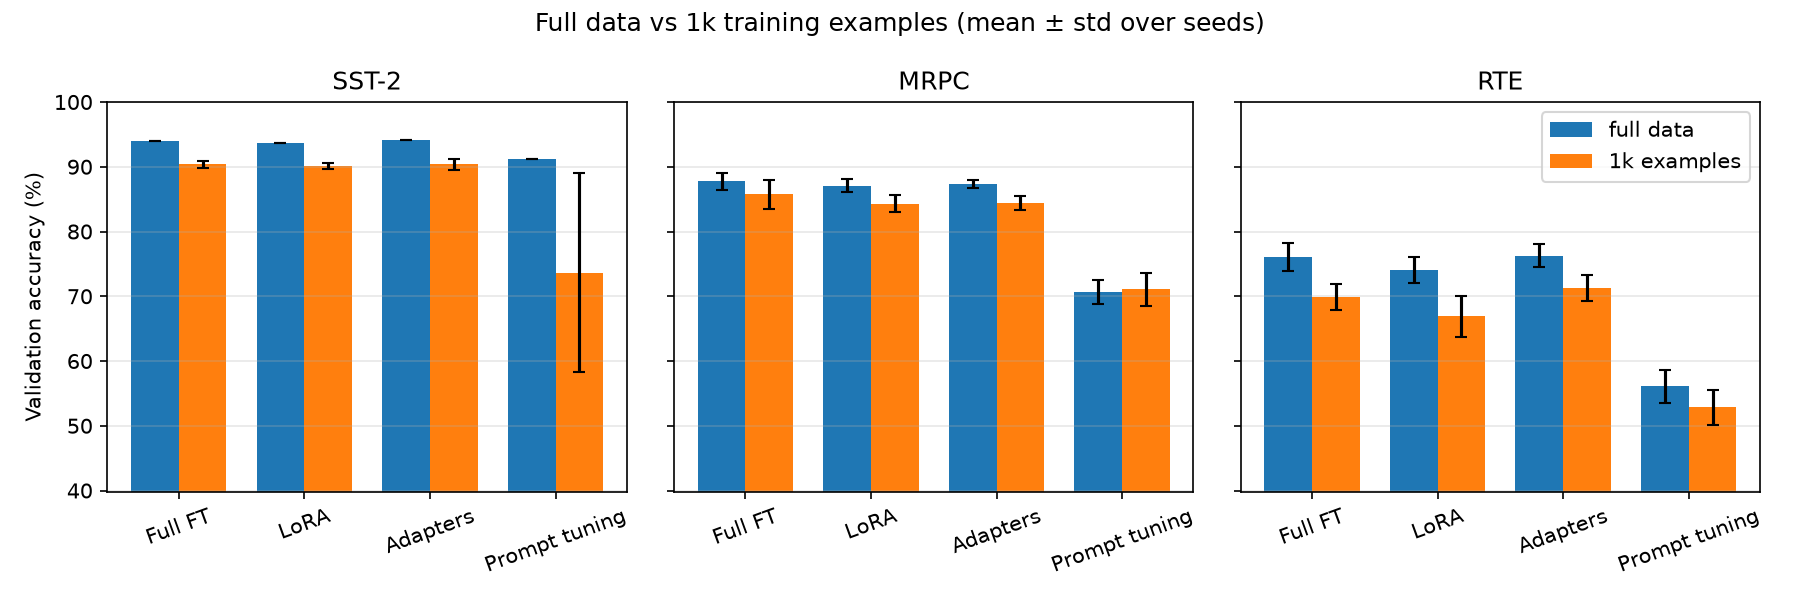
\includegraphics[width=\columnwidth]{figures/full_vs_1k.png}
\caption{Validation accuracy with full training data vs 1,000 examples, per method and task.}
\label{fig:lowdata}
\end{figure}

\subsection{Ablations}

\begin{table}[t]
\centering
\small
\begin{tabular}{@{}llrr@{}}
\toprule
Method & Setting & RTE acc & Params \\
\midrule
Full FT & 0 frozen (default) & 76.1 $\pm$ 2.2 & 124.6M \\
 & 3 frozen & 75.2 $\pm$ 0.8 & 64.4M \\
 & 6 frozen & 73.0 $\pm$ 1.8 & 43.1M \\
 & 9 frozen & 65.3 $\pm$ 1.7 & 21.9M \\
\midrule
LoRA & $r{=}1$ & 70.0 $\pm$ 1.4 & 0.63M \\
 & $r{=}4$ & 72.0 $\pm$ 3.7 & 0.74M \\
 & $r{=}8$ (default) & 74.0 $\pm$ 2.0 & 0.89M \\
 & $r{=}16$ & 74.4 $\pm$ 0.0 & 1.18M \\
 & $r{=}64$ & 60.0 $\pm$ 10.3 & 2.95M \\
\midrule
Adapters & Houlsby, rf 8 & 77.6 $\pm$ 1.9 & 4.15M \\
 & Houlsby, rf 16 (default) & 76.3 $\pm$ 1.8 & 2.38M \\
 & Houlsby, rf 64 & 70.2 $\pm$ 2.9 & 1.05M \\
 & Pfeiffer, rf 16 & 74.1 $\pm$ 3.6 & 1.49M \\
\midrule
Prompt & 5 tokens & 52.3 $\pm$ 2.5 & 0.60M \\
tuning & 20 tokens (default) & 56.1 $\pm$ 2.6 & 0.61M \\
 & 50 tokens & 53.2 $\pm$ 4.2 & 0.63M \\
 & 100 tokens & 52.6 $\pm$ 1.6 & 0.67M \\
 & 20 tokens, text init & 53.8 $\pm$ 1.6 & 0.61M \\
\bottomrule
\end{tabular}
\caption{Ablations on RTE (full data), validation accuracy $\times$100, mean $\pm$ std over 3 seeds. ``Frozen'' = embeddings and the bottom $k$ layers frozen; rf = reduction factor. LoRA keeps $\alpha{=}2r$.}
\label{tab:ablation}
\end{table}

Each ablation changes one setting of one method, on RTE with full data and seeds 1--3 (Table~\ref{tab:ablation}, Figure~\ref{fig:ablation}). The default row is the final run, and the learning rate is unchanged.

\paragraph{Partial Full FT is a poor alternative to PEFT.} Freezing the bottom 9 layers still trains 21.9M parameters but drops RTE accuracy to 65.3\%. LoRA trains 25 times fewer parameters and reaches 74.0\%. Freezing 3 layers keeps most of the accuracy (75.2\%) with 28\% less memory than Full FT (2,349\,MiB), but it still uses more memory than any PEFT method.

\paragraph{LoRA rank.} Accuracy rises from $r{=}1$ (70.0) to $r{=}8$--16 (74.0--74.4) and collapses at $r{=}64$, where two of three seeds stayed at majority-class level (52.7\% and 55.6\%) while the third reached 71.8\%. With $\alpha{=}2r$, 5e-4 appears too high a learning rate for $r{=}64$. We did not re-tune it per rank, so this shows instability at a fixed learning rate. It does not show that high ranks are worse in general.

\paragraph{Adapter size and type.} A larger bottleneck helps: reduction factor 8 reaches 77.6\%, the best RTE score in the study, with 4.2M trainable parameters and almost no extra memory. Reduction factor 64 loses 6 points. At the same reduction factor, the Pfeiffer configuration is 2.2 points below Houlsby, with 38\% fewer trainable parameters.

\paragraph{Prompt length and initialisation.} No setting moves prompt tuning more than 3.4 points above the majority class. Longer prompts make every input longer, so memory and time grow with prompt length (100 tokens: 2,626\,MiB and 175\,s) without any gain in accuracy. Initialising the prompt from a short text did not help either (53.8 vs 56.1).

\begin{figure*}[t]
\centering
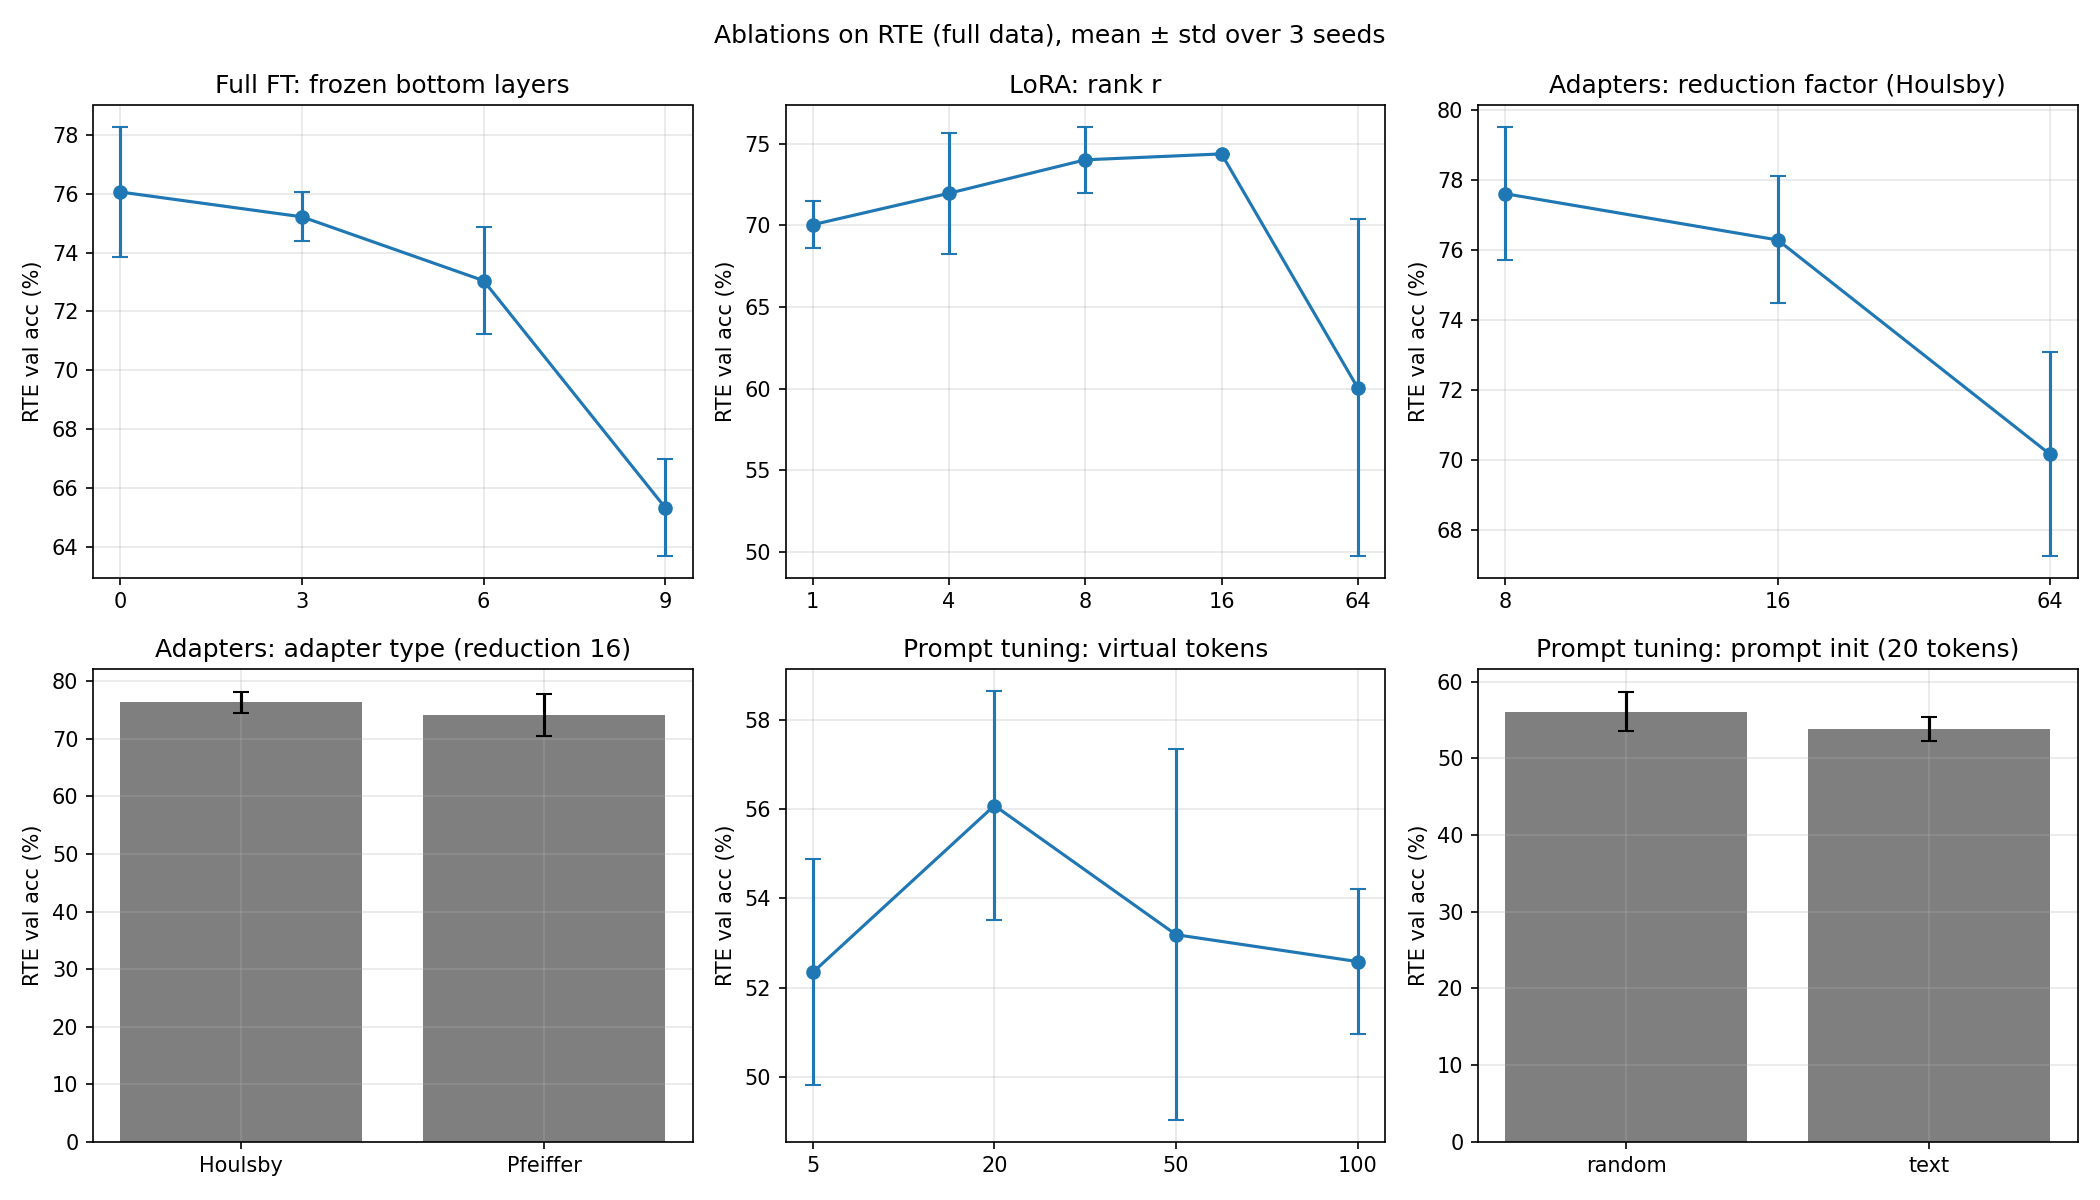
\includegraphics[width=0.9\textwidth]{figures/ablations.png}
\caption{Ablations on RTE (full data), mean $\pm$ std over 3 seeds.}
\label{fig:ablation}
\end{figure*}

\section{Discussion}

\paragraph{Why prompt tuning is weak on \texttt{roberta-base}.} Prompt tuning trains only 15,360 prompt parameters and changes the model's behaviour only through attention to those 20 positions. \citet{lester2021} found that this works only when the frozen model is very large: for T5, prompt tuning matched full fine-tuning only at about 11B parameters. \texttt{roberta-base} has 125M parameters, so our results agree with that finding. Our ablations show that the problem is not the prompt length or the initialisation. Prompt tuning did learn SST-2 with 67k examples, but two tasks are too hard for it at this scale and budget: sentence-pair inference with 2.5k examples (RTE) and paraphrase detection with 3.7k examples (MRPC).

\paragraph{Why adapters can match Full FT.} RTE and MRPC have only a few thousand training examples, and Full FT overfits easily on them (RTE dev accuracy varies by $\pm$4.4 points across seeds). Adapters keep the pretrained weights fixed and add a small change to each layer, which limits how far the model can move from its pretrained state. The ablations show that capacity still matters: reduction factor 8 helped and 64 hurt.

\paragraph{Recommendations.} Under a memory limit, use adapters or LoRA: about 1.9\,GB peak vs 3.3\,GB for Full FT, losing at most 2.1 points. Under a time limit, use LoRA on large datasets (324 vs 492\,s on SST-2) and adapters on small ones (106 vs 158\,s on RTE). With very little data, use adapters or Full FT, and avoid prompt tuning. To serve many tasks from one model, LoRA needs 3.4\,MB per task and can be merged into the weights, so inference costs nothing extra.

\section{Conclusion}

With one shared budget on \texttt{roberta-base}, adapters and LoRA keep almost all of Full FT's accuracy on SST-2, MRPC and RTE. They train 0.7--1.9\% of the parameters, use about 40\% less GPU memory and need 3--9\,MB per task instead of 475\,MB. With 1,000 training examples, Full FT and adapters lose the least accuracy. Prompt tuning has the smallest checkpoint, but at this model size it stays near the majority-class baseline on MRPC and RTE and is unstable with little data. Freezing layers of Full FT is a much worse trade-off than either LoRA or adapters.

\section*{Limitations}

SST-2 full data has only one seed per method, so the SST-2 full numbers have no standard deviation and should not be read as a ranking. Three seeds are few for RTE and MRPC, and many of our differences are smaller than one standard deviation. The LR search was run after the final runs with seed 1 only. The ablations are on RTE only, and the learning rate was not re-tuned per setting, which matters most for LoRA $r{=}64$. All methods get the same number of epochs, but prompt tuning was often still improving at the last epoch. The 10\% dev split is drawn with the run's seed, so dev accuracy varies more than validation accuracy. Peak memory is \texttt{max\_memory\_allocated}, which leaves out the allocator cache. Adapters use AdapterHub instead of Hugging Face PEFT, because PEFT has no Houlsby adapters. We report on the GLUE validation split because test labels are hidden. The validation split was never used for any choice.

\section*{Team Contributions}

Deepak Mandal: full fine-tuning (16 runs), repository, data pipeline, training and Kaggle run scripts. Anoop Kumar: LoRA (16 runs), results format and validation, analysis notebook, LR search and ablation runs. Chiranjeet Biswas: adapters (16 runs), background and literature review. Byagari Praveen Kumar: prompt tuning (16 runs), results tables, plots and slides.

\bibliography{custom}

\end{document}
